% !TEX TS-program = pdflatex
% !TEX encoding = UTF-8 Unicode

% This is a simple template for a LaTeX document using the "article" class.
% See "book", "report", "letter" for other types of document.

\documentclass[11pt]{report} % use larger type; default would be 10pt

\usepackage[utf8]{inputenc} % set input encoding (not needed with XeLaTeX)
\usepackage{float}
\usepackage{tabularx}

%%% Examples of Article customizations
% These packages are optional, depending whether you want the features they provide.
% See the LaTeX Companion or other references for full information.

%%% PAGE DIMENSIONS
\usepackage{geometry} % to change the page dimensions
\geometry{a4paper} % or letterpaper (US) or a5paper or....
% \geometry{margin=2in} % for example, change the margins to 2 inches all round
% \geometry{landscape} % set up the page for landscape
%   read geometry.pdf for detailed page layout information

\usepackage{graphicx} % support the \includegraphics command and options

% \usepackage[parfill]{parskip} % Activate to begin paragraphs with an empty line rather than an indent

%%% PACKAGES
\usepackage{booktabs} % for much better looking tables
\usepackage{array} % for better arrays (eg matrices) in maths
\usepackage{paralist} % very flexible & customisable lists (eg. enumerate/itemize, etc.)
\usepackage{verbatim} % adds environment for commenting out blocks of text & for better verbatim
\usepackage{subfigure} % make it possible to include more than one captioned figure/table in a single float
% These packages are all incorporated in the memoir class to one degree or another...

%%% HEADERS & FOOTERS
\usepackage{fancyhdr} % This should be set AFTER setting up the page geometry
\pagestyle{fancy} % options: empty , plain , fancy
\renewcommand{\headrulewidth}{0pt} % customise the layout...
\lhead{}\chead{}\rhead{}
\lfoot{}\cfoot{\thepage}\rfoot{}

%%% SECTION TITLE APPEARANCE
\usepackage{sectsty}
\allsectionsfont{\sffamily\mdseries\upshape} % (See the fntguide.pdf for font help)
% (This matches ConTeXt defaults)

%%% ToC (table of contents) APPEARANCE
\usepackage[nottoc,notlof,notlot]{tocbibind} % Put the bibliography in the ToC
\usepackage[titles,subfigure]{tocloft} % Alter the style of the Table of Contents
\renewcommand{\cftsecfont}{\rmfamily\mdseries\upshape}
\renewcommand{\cftsecpagefont}{\rmfamily\mdseries\upshape} % No bold!

%%% Share Figure and Table Numbering %%%
\makeatletter
\renewcommand*{\thetable}{\arabic{table}}
\renewcommand*{\thefigure}{\arabic{figure}}
\let\c@table\c@figure

%%% Code Listings %%%
\usepackage{color}
\usepackage{listings}

\definecolor{dkgreen}{rgb}{0,0.6,0}
\definecolor{gray}{rgb}{0.5,0.5,0.5}
\definecolor{mauve}{rgb}{0.58,0,0.82}
\lstset{
  language=Python,
  showstringspaces=false,
  formfeed=\newpage,
  tabsize=2,
  commentstyle=\itshape,
  basicstyle=\ttfamily,
  morekeywords={models, lambda, forms},
keywordstyle=\color{blue},          % keyword style
  commentstyle=\color{dkgreen},       % comment style
  stringstyle=\color{mauve},         % string literal style
frame=shadowbox,
breaklines=true
}


\usepackage[parfill]{parskip} % Uncomment this to have no paragraph indentation
\usepackage{mathtools}
\usepackage[english]{babel}
\usepackage{graphicx}
\usepackage{tikz}
% \usepackage{subfigure}
\usetikzlibrary{positioning}
\usetikzlibrary{shapes,arrows}
%%% END Article customizations



%%% The "real" document content comes below...

\title{Automatic Star-rating Generation from Text Reviews}
\author{
  Chong-U Lim\\
  \texttt{culim@csail.mit.edu}
  \and
  Pablo Ortiz\\
  \texttt{portiz@csail.mit.edu}
  \and
 Sang-Woo Jun\\
  \texttt{wjun@csail.mit.edu}
}
%\date{} % Activate to display a given date or no date (if empty),
         % otherwise the current date is printed 

\begin{document}
\maketitle

\tableofcontents

\newpage
\chapter{Background}
\section{Introduction}
For our final project, we designed a system that generates five-star ratings for a product based on a review of that product. Ratings are generated by classifying the overall sentiment of a product review on the five-star scale using an adaptation of the PMI-IR algorithm. In the actual implementation of the system, we constrained the domain of product reviews to those of mobile applications on the Google Play App store. It was necessary to constrain the system to a particular problem domain as different problem domains will produce different sentiments for the same words. The system we created can serve as a proof of concept for generating five-star ratings based on product reviews for products and services of various kinds.

\section{Motivation}
Accurate customer feedback is much sought after by commercial enterprises. The information is quite valuable and affects a comapny's bottom line by aiding in the design of new products/services or helping to fix those that have not been well-received. This being the  case, many companies invite their customers to submit reviews for products they have used. The format of these reviews can vary widely from the ``Like" format used by Facebook to lengthy surveys. Some formats, of course, are used more in practice than others.

One well-established format for customer reviews is that of five-star ratings paired with short text reviews. Feedback in this form allows a customer to both give an overall rating for a product/service and provide meaningful commentary about the product/service. Unfortunately, a problem related to the accuracy of the reviews comes up when feedback is formatted this way. A particular star rating can mean completely different things to two different customers. For example, suppose there is one customer who sees the world in black and white and another customer who sees the world along the full five-star gradient. A one-star review from the first customer could mean anything between minor dislike and absolute hatred. The content of this customer's text review would likely give others greater insight into the exact amount of dislike behind the rating. A one-star review from the second customer would always indicate absolute hatred. The content of this customer's text review would simply re-enforce the intent of their rating. Though this example is quite extreme, it illustrates a flaw inherent to this system of obtaining feedback: some star ratings will not match the corresponding sentiment seen in the accompanying text commentary. For a commercial enterprise looking to collect accurate feedback from its customer reviews, this should be a matter of much concern.

To acquire more accurate information from customer feedback, we propose the removal of five-star ratings from these review formats entirely. Instead, we propose that the star-ratings be generated in a uniform fashion from the sentiment of the text commentary.

\section{Previous Work}

Our focus in this work is using sentiment analysis to determine the polarity of
natural language sentences. For example, classifying them into either positive
or negative classes. This is a subset of sentiment analysis that is recently
gathering interest, with the increasing popularity of product review sites such
as Amazon. However, attempts to extract features or information from natural
language sentences have a long history.

SVMs have been traditionally been used for language classification. For example,
Joachims have lead an early research in using SVMs for text
classification~\cite{Joachims:1998:TCS:645326.649721}. A similar work in genre
detection was done using neural networks and surface
cues~\cite{Kessler:1997:ADT:976909.979622}. A deeper analysis of context was
attempted by Snyder \cite{Snyder07multipleaspect}.

With the growth of review sites such as Amazon and Youtube, there has been
growing popularity of study on the polarity of the sentences. Turney led the
initial research on extracting polarity of texts~\cite{Turney2001,
Pang:2002:TUS:1118693.1118704}. The focus on multi-level star ratings has also
been explored in depth~\cite{Pang+Lee:05a}.


\section{Contributions}

In this work, we explore multiple methods for generating the star-ratings of prodcut/service reviews. Of these methods, the best one we assessed uses a novel approach for determining the underlying sentiment of a passage of text. The star-ratings generated from this method using mobile application reviews perform comparably with the performance of the PMI-IR method in the context of movie reviews.

%%% BEGIN Chapter: Design
\chapter{Design}
\section{Data Collection}

\begin{figure}[h!]
  \centering
    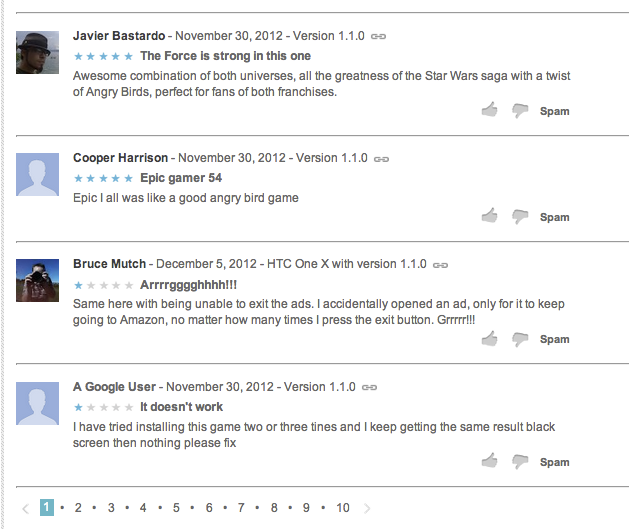
\includegraphics[width=0.6\textwidth]{figures/playstore.png}
 \caption{User Reviews on the Google Play Store}
\label{fig:playstore}
\end{figure}

Google does not supply any publicly available Application Programming Interfaces (APIs) to query for data or results on the Google Play Store. Also, in searching for user reviews for a given application, one has to first navigate to the associated page and is at first initially presented with only the first 10 reviews, with the rest only asynchronously provided when a user clicks on the paginated links at the bottom (Figure~\ref{fig:playstore}). 

\begin{figure}[h!]
  \centering
    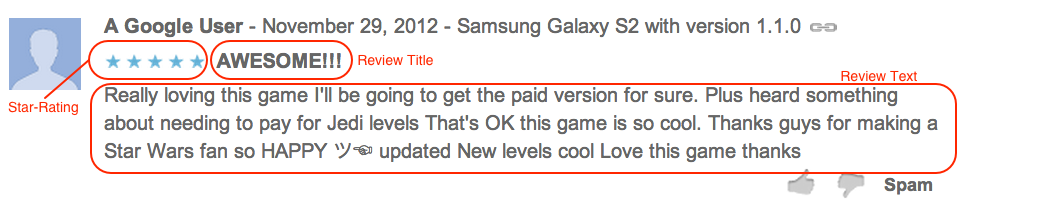
\includegraphics[width=0.8\textwidth]{figures/user_review.png}
 \caption{User Reviews on the Google Play Store}
\label{fig:user_review}
\end{figure}

However, attempts to automated the querying for more results were blocked by Google. As such, we had to manually obtain the data by first clicking through all the provided pagination links at the bottom in order to load all the user reviews. After which, we made use of Google Chrome's View Source functionality to extract all DOM elements between the \verb|<html>| element. A python script was then used to locate each user review, and extract out 3 main features, namely, the \textbf{Review Title}, \textbf{Review Text} and the \textbf{Star-Rating} (Figure~\ref{fig:user_review}).

\section{Phrase Extraction}
\label{subsection:phrase_extraction}
\subsection{Parts-Of-Speech (POS) Tagging}
The text gathered as part of the \textbf{review text} often varies in length (i.e. number of sentences, number of words). Our aim is to extract out the important phrases in each review and use them to guide our calculation of the overall sentiment of the user's review. In order to do so, we first process the review text by splitting them into sentences, followed by determining the part-of-speech (POS) tags for each word in the sentence. 
\subsection{Pattern Matching}
\begin{table}[h]
	\centering
    \begin{tabular}{  l  l  l  l}
    \hline\hline
    	 & First Word & Second Word & \shortstack{Third Word \\ (Not Extracted} \\ \hline
	1. & JJ, JJS, JJR & NN, NNS & anything \\ \hline
	2. & RB, RBR, RBS &JJ, JJS, JJR & neither NN nor NNS \\ \hline
	3. & JJ, JJS, JJR & JJ, JJS, JJRS & neither NN nor NNS \\ \hline
	4. & NN, NNS & JJ, JJS, JJRS & neither NN nor NNS \\ \hline
	5. & RB, RBR, RBS &VB, VBD, VBN, VBG & anything \\ \hline
	6. & DT & JJ, JJS, JJRS & anything \\ \hline
	7. & VBZ & JJ, JJS, JJRS & anything \\ \hline
    \hline
    \end{tabular}
\caption{Patterns of POS Tags for 2-Word Phrase Extraction}
\label{fig:postags}
\end{table}

Given the tokenized form of the sentence, we proceed to extract 2-word phrases from the review via pattern matching against a set of phrase patterns, as shown in Table~\ref{fig:postags}. The patterns of POS tags are extended from an original list proposed by Turney~\cite{Turney2001}. Our extensions were required in order to better match style of reviews on the Google Play Store, and also to match the tokens used in the \textit{NLTK} library. One notable addition was the addition of \textit{superlative} adjectives (JJS), which we were emperically found to occur substantially in our dataset, with sentences such as `` \textit{\dots this game is \textbf{the best} ! \dots}." We also added comparative adjectives (JJS) to our matched tags. Figure~\ref{fig:phrase_extraction} shows the results of our phrase extraction on a user review in our dataset.

\begin{figure}[h!]
  \centering
\begin{lstlisting}
text = "This is a great game but lags horribly. I'm constantly dying because it freezes up on me! Pleasseee do something to fix it!:)"
>>> get_phrases_from_text(text)
[[('a', 'DT'), ('great', 'JJ')], [('great', 'JJ'), ('game', 'NN')], [('constantly', 'RB'), ('dying', 'VBG')]]

\end{lstlisting}
 \caption{User Reviews on the Google Play Store}
\label{fig:phrase_extraction}
\end{figure}

\section{Phrase Sentiment}
\label{section:phrase_sentiment}
In order to gain insight regarding the user's sentiment based on his or her review, we make use of the extracted phrases from 
Section~\ref{subsection:phrase_extraction} as a measure of a user's sentiment towards the application. The basis of extracting information from the phrases is derived from the mutual information of the words contained within the phrase, against known words that we identified as having either \textit{positive} or \textit{negative} sentiment polarity. 

\subsection{Pointwise Mutual Information (PMI)}
The Pointwise Mutual Information (PMI) between two words \cite{church1990} is defined with the following equation:

% \begin{math}...\end{math}
\begin{equation*} PMI(word_1, word_2) = \log_2 \left(\frac{Pr[word_1 \: and \: word_2]}{Pr[word_1] \times Pr[word_2]}\right) \end{equation*}

In the equation, the term $Pr[word]$ refers to the probability of the word appearing if we were to sample randomly from a text corpus, while  $Pr[word_1 \: and \: word_2]$ refers to the probability of both words appearing together. The ratio between p(word1 \& word2) and p(word1) p(word2) is thus a measure of the degree of statistical dependence between the words. The log of this ratio is the information gain from one of the words when the other is observed. The PMI score has an additional property in which it assigns a proportionally higher score to the words that appear infrequently in a given corpus, but with a higher likelihood of appearing together in the event they do. \cite{Vargas2010} 

\subsection{Semantic Orientation}
The semantic orientation of a given phrase is thus given by the formula:
\begin{equation*} SO(phrase) = PMI(phrase, \verb|<positive>|) - PMI(phrase, \verb|<negative>|)\end{equation*}

In the formula, the terms \verb|positive| and \verb|negative| refer to words which are respectively associated with positive sentiments and negative sentiments. 

\subsection{PMI-IR}
In Turney's implementation, he made used of the the words \textit{"excellent"} and \textit{"negative"}. Also, he introduces a technique called PMI-IR (Information Retrieval) in order to estimate the PMI values by using hit counts returned from search engine queries. He estimates the semantic orientation using the formula:

\begin{equation*} SO(phrase) = \log_2 \left(\frac{hits(phrase \: NEAR \: ``excellent") \times hits(``poor") }{hits(phrase \: NEAR \: ``poor") \times hits(``excellent") }\right) \end{equation*}

The term \textit{NEAR} in the equation above is a search query modifier which only returns results in which the items are located within a fixed number of words between each other. 

As a basis for our implementatiiorion, we used a similar PMI-IR estimation for semantic orientation of the extracted phrases, but using Google as the search engine of choice, and replacing the \textit{NEAR} operator with Google's corresponding \textit{AROUND(n)} operator (where \text{n} indicates the maximum range of words of which the two items in the search could differ by.)

However, based on our initial findings, we identified two problems with this approach. Firstly, automated queries to Google go against its Terms of Service Agreement. Despite attempts to decrease the likelihood of being detected such as by limiting our queries to a random interval between 10-15 seconds, we got blocked after about 50-60 calls. A survey of other alternative search engines either resulted in similar limits enforced (Bing), or deprecated APIs (Yahoo, Altavista). This made the process a slow and cumbersome endeavour.

The second problem was associated with the accuracy of the calculated results, which are outlined in greater detail in Chapter~\ref{chapter:results}. In short, the results failed to convincingly associate phrases with the correct polarity, partly due to the fact that the Google Search API does not actually return accurate values for the number of hits.

\subsection{Corpus-Derived PMI}
We began looking at offline methods of calculating semantic orientation values. We settled on somehow making use of a corpus in a similar problem domain as the one we were analyzing (\textit{NLTK} \verb|movie_reviews|) to calculate semantic orientation values for words, phrases, and sentences. 

\subsubsection{PMI-Concordance}
In our first experiment, we tried using the concordance of words in the movie review corpus to calculate the semantic orientation of words, phrases, and, sentences in a small data set. By concordance, we mean the measure of the relative distance between two words in a document. We thought this metric might act as a good substitute for search engine hit counts for comparing how close a particular word is in meaning to a known, very positivel or negativel polarized word. This turned out to slightly better than the PMI-IR approach in terms of accuracy, but the calculations took a  long time to process.

\subsubsection{PMI-CUE}
In order to find a method of calculating SO scores for phrases quickly, and without limit, we turned towards an offline SO estimator which uses the \textit{NLTK} \verb|movie_reviews| corpus. We term it the PMI-CUE (Corpus Underlying Estimator). The corpus is a collection of user reviews from the \textit{IMDB Movie Database} , and is separated into sentences associated with \textit{positive} and \textit{negative} reviews. In our implementation, we first created a probability distribution of words which appear in the \text{positive} reviews and \text{negative} reviews separately. Next, we estimated the semantic orientation of a phrase using the formula:

\begin{equation*} SO(word) = \log_2 \left(\frac{Pr_{pos}[word]}{Pr_{neg}[word]}\right) \end{equation*}

Where the term $Pr_{pos}[word]$ is the probability of occurence of the word $word$ using the frequency distribution model acquired from the \textit{positive} corpus. The term $Pr_{pos}[word]$ naturally refers to the corresponding definition associated with the \textit{negative} corpus. We can easily extend this to a phrase with two words, such as ``very annoying" by calculating $SO(``very") + SO(``annoying")$. This allows us to attain values such as $SO(`excellent`")=1.2432$, $SO(``poor")=-0.9219$, $SO(``very \: annoying")=-0.3952$ and $SO(``very \: happy")=0.6716$. Thus, this gives us a nice form in which positive phrases are given positive values, and negative phrases are given negative values. Also, the magnitude of a value indicates a stronger association with the polarity.

\subsection{Text Semantic Orientation}
Given that a review text often contains several sentences, which in part contain several phrases which match our phrase patterns, we calculate the semantic orientation of a given text by averaging the semantic orientation values of its constituent matched-phrases. We present the calculation of two reviews from our dataset, one corresponding to a positive user review (Figure~\ref{fig:positive_review}) and another corresponding to a negative user review (Figure~\ref{fig:negative_review}). We illustrate the phrase extracted together with its constituent POS tags and the results of the per-phrase semantic-orientation calculation and overall semantic orientation of the review.

\pagebreak
\subsubsection{Positive Review}
\begin{comment}
pprint(res_free[130])
{'original_index': 32,
 'phrases': [[(u'is', 'VBZ'), (u'such', 'JJ')],
             [(u'an', 'DT'), (u'entertaining', 'JJ')],
             [(u'entertaining', 'JJ'), (u'game', 'NN')],
             [(u'is', 'VBZ'), (u'great', 'JJ')],
             [(u'Another', 'DT'), (u'great', 'JJ')]],
 'rating-calculated': 5.0,
 'rating-user': 5.0,
 'so': 0.4126400904562006,
 'text': u'This is such an entertaining game that is great for killing time. Another great Angry Birds game :-)',
 'text-cls': 'pos',
 'title': u'Fantastic Game',
 'title-cls': 'pos'}

>>> so_2("is", "such")
0.15734872244647513
>>> so_2("an", "entertaining")
0.32014397089151714
>>> so_2("entertaining", "game")
0.385981805784978
>>> so_2("is", "great")
0.6650209890754402
>>> so_2("another", "great")
0.4515674226156673
\end{comment}
\begin{table}[h!]
	\centering
    \begin{tabular}{  l  l  c}
    \hline\hline
    	 Extracted Phrase & POS Tags & Semantic Orientation \\ \hline
	is such & VBZ JJ & 0.1573 \\ \hline
	an entertaining & DT JJ & 0.3201 \\ \hline
	entertaining game & JJ NN & -0.1939 \\ \hline \hline
	is great & VBZ JJ & 0.6650 \\ \hline \hline
	another great & DT JJ & 0.4515 \\ \hline \hline
	Average Semantic Orientation & & 0.4126\\ \hline
    \hline
    \end{tabular}
\caption{Semantic Orientation Calculation for a Positive Review}
\label{fig:positive_review}
\end{table}


\subsubsection{Negative Review}
\begin{comment}
pprint(bad_free[55])
{'original_index': 936,
 'phrases': [[(u'a', 'DT'), (u'big', 'JJ')],
             [(u'big', 'JJ'), (u'fan', 'NN')],
             [(u'a', 'DT'), (u'huge', 'JJ')],
             [(u'huge', 'JJ'), (u'problem', 'NN')],
             [(u"n't", 'RB'), (u'work', 'VB')],
             [(u'even', 'RB'), (u'uninstalled', 'VBD')],
             [(u'then', 'RB'), (u'reinstalled', 'VBD')],
             [(u'again', 'RB'), (u'help', 'VB')],
             [(u"n't", 'RB'), (u'stay', 'VB')]],
 'rating-calculated': 1.0,
 'rating-user': 2.0,
 'so': -0.29789422119460257,
 'text': u"I love this game a lot! I'm a big fan and an addict to this game but recently I have been Facing a huge problem now I open this game it doesn't work it opens and then closes straight away I even uninstalled it and then reinstalled it but no difference same thing again help me please I love this can't stay without playing it",
 'text-cls': 'neg',
 'title': u'Fix it !!!',
 'title-cls': 'neg'}

>>> so_2("a", "big")
-0.33098922965584293
>>> so_2("big", "fan")
-0.7056408179636935
>>> so_2("a", "huge")
-0.23955015985152298
>>> so_2("huge", "problem")
-0.7483314776169897
>>> so_2("not", "work")
-0.06760705836956686
>>> so_2("even", "uninstalled")
-0.26451873835339673
>>> so_2("then", "reinstsalled")
-0.3341268897682953
>>> so_2("again", "help")
0.07927221248239999
>>> so_2("not", "stay")
-0.06955583165451482

\end{comment}
\begin{table}[h]
	\centering
    \begin{tabular}{  l  l  c }
    \hline\hline
    	 Extracted Phrase & POS Tags & Semantic Orientation \\ \hline
	 a big & DT JJ & -0.3309 \\ \hline
	big fan & JJ NN & -0.7056 \\ \hline
	a huge & DT JJ & -0.2395 \\ \hline \hline
	huge problem & JJ NN & -0.7483 \\ \hline \hline
	not work &  RB VBD & -0.0676 \\ \hline \hline
	even uninstalled & RB VBD  & -0.2645 \\ \hline \hline
	then reinstalled &  RB VBD & 0.3341 \\ \hline \hline
	again help &  RB VB  & 0.0792 \\ \hline \hline
	not stay & RB VB & -0.0695\\ \hline \hline
	Average Semantic Orientation & & -0.2978 \\ \hline
    \hline
    \end{tabular}
\caption{Semantic Orientation Calculation for a Negative Review}
\label{fig:negative_review}
\end{table}

\section{Text Polarity}
\label{section:text_polarity}
\subsection{Bag of Words}
A second method into gaining insight into the sentiments expressed within a sentence is to determine its polarity. The polarity may be either \textit{positive} or \textit{negative}, and it treats polarity using the \textbf{Bag of Words} (BOW) model~\cite{harris1954}. In this model, a document is represented by the occurrences of words in it regardless their position in the document. This is implemented with the \textit{NLTK} \verb|movie_reviews| corpus by creating feature vectors based on the appearance of words in each sub-corpus, with each sub-corpus forming a single training instance. We do this separately for both the \textit{positive} and \textit{negative} categories. 

\subsection{Naive Bayes Classifier}
Classification is then performed by a Naive Bayes classifier~\cite{lewis1998naive, mccallum1998comparison} using the feature vector of word-appearances, using the following approximation:

\begin{equation*} Pr[polarity | w_1, \dots, w_n] 	\approx	 Pr[polarity]  \prod_{n=1}^nPr[w_i|polarity] \end{equation*}

The LHS of the equation is the probability of the polarity taking a certain value conditioned on the joint probability of occurrence of a given sequence of words $w_1, \dots, w_n$. By using Bayes' Theorem, the result of the equation can be re-written based on the prior probability of attaining a certain polarity classificaiton $Pr[polarity]$, and the conditional polarity of generating a sequence of words $w_1, \dots, w_n$ given a known polarity. By assuming conditional independence of the appearance of each word $w_i$ given a $polarity$, we may represent the joint conditional probability as a product of individual probabilities of the occurrence of a word $w_i$ given a $polarity$, $Pr[w_i|polarity]$, thus revealing the formula on the RHS of the equation.

\begin{table}[h]
	\centering
    \begin{tabular}{  c || c  c  c  c  c ||  c  }
    \hline\hline
    	 fileid & \dots & abberline & ably & achieve &\dots & category \\ \hline
	 \verb|pos/cv000_29590.txt|& \dots & \verb|true| & \verb|true| & \verb|false| &\dots & \verb|positive| \\ \hline
	 \verb|pos/cv001_18431.txt|& \dots & \verb|false| & \verb|false| & \verb|true| &\dots & \verb|positive| \\ \hline
	 \vdots & \vdots  & \vdots  & \vdots & \vdots &\vdots & \vdots \\ \hline
	 \verb|neg/cv999_14636.txt|& \dots & \verb|false| & \verb|false| & \verb|false| &\dots & \verb|negative| \\ \hline


    \hline
    \end{tabular}
\caption{Constructing Naive Bayes Training Data from NLTKs movie\_reviews corpus}
\label{fig:naivebayes}
\end{table}

The \textit{NLTK} \verb|movie_reviews| corpus contains 1000 files associated with the \textit{positive} sentiment, and 1000 files associated with the \textit{negative} sentiment (identified by the category type \verb|"pos"| and \verb|"neg"|.) Table~\ref{fig:naivebayes} shows how the training data was constructed using the \verb|movie_reviews| corpus. Figure~\ref{fig:naivebayes_classifying_review} illustrates the process of determining the polarity of a user's review. The text is first tokenized into individual word tokens and then converted into a feature vector. Finally, our classifier is used to classify the feature vector, in which it calculates the label \verb|neg|, indicating a negative polarity in the user's review.

\begin{figure}[h!]
  \centering
\begin{lstlisting}
>>> sample_text
u'I was fine with having to exit ads on previous Angry Birds games, but this is a two -step requirement. You have to expand first and then exit the ad, and for me, using a Samsung Galaxy S3, it will only take me to the ad link when I touch the X. Broken ad exit button will not let me play. Uninstalling.'

>>> sample_text_tokens
['I', 'was', 'fine', 'with', 'having', 'to', 'exit', 'ads', 'on', 'previous', 'Angry', 'Birds', 'games', ',', 'but', 'this', 'is', 'a', 'two', '-step', 'requirement.', 'You', 'have', 'to', 'expand', 'first', 'and', 'then', 'exit', 'the', 'ad', ',', 'and', 'for', 'me', ',', 'using', 'a', 'Samsung', 'Galaxy', 'S3', ',', 'it', 'will', 'only', 'take', 'me', 'to', 'the', 'ad', 'link', 'when', 'I', 'touch', 'the', 'X.', 'Broken', 'ad', 'exit', 'button', 'will', 'not', 'let', 'me', 'play.', 'Uninstalling', '.']

>>> text_features = word_feats(sample_text_tokens)
{'and': True, 'ad': True, 'S3': True, 'Angry': True, 'it': True, 'two': True, 'have': True, 'touch': True, 'You': True, 'fine': True, 'previous': True, '-step': True, 'X.': True, 'ads': True, 'for': True, 'Broken': True, 'when': True, ',': True, '.': True, 'to': True, 'only': True, 'exit': True, 'take': True, 'was': True, 'is': True, 'then': True, 'Samsung': True, 'I': True, 'but': True, 'me': True, 'link': True, 'play.': True, 'not': True, 'using': True, 'let': True, 'with': True, 'expand': True, 'a': True, 'on': True, 'Uninstalling': True, 'this': True, 'button': True, 'having': True, 'will': True, 'games': True, 'requirement.': True, 'the': True, 'Birds': True, 'Galaxy': True, 'first': True}

>>> classifier.classify(text_features)
"neg"

\end{lstlisting}
 \caption{User Reviews on the Google Play Store}
\label{fig:naivebayes_classifying_review}
\end{figure}

\section{Hierarchical Classification}
In our implementation, we aimed to provide a way to make use of both the semantic orientation (Section~\ref{section:phrase_sentiment}) and the polarity(Section~\ref{section:text_polarity}) of a user review in order to generate more accurate reviews on a 5-star rating scale. The approach we took makes use of a \textbf{Hierarchical Classifier}~\cite{ruiz2002hierarchical,sun2001hierarchical} in which the review to be classified is first classified based on its polarity. Next, we predict the exact star-rating based on the semantic-orientation of the review's extracted phrases.

% Define block styles
\tikzstyle{decision} = [diamond, draw, fill=blue!20, 
    text width=4.5em, text badly centered, node distance=3cm, inner sep=0pt]
\tikzstyle{block} = [rectangle, draw, fill=blue!20, 
    text width=5em, text centered, rounded corners, minimum height=4em]
\tikzstyle{line} = [draw, -latex']
\tikzstyle{cloud} = [draw, ellipse,fill=red!20, node distance=3cm,    minimum height=2em]
\tikzstyle{smallcloud} = [draw, circle ,fill=yellow!20, minimum height=3em]
\begin{figure}[h!]
\center
\begin{tikzpicture}[node distance = 2cm, auto]
    % Place nodes
    \node [block] (init) {text-polarity};
    \node [cloud, below left of=init] (negative) {negative};
    \node [cloud, below right of=init] (positive) {positive};
	\node [block, below of=negative] (so-neg) {semantic orientation};
	\node [block, below of=positive] (so-pos) {semantic orientation};
\node [smallcloud, below left=1cm and 1.0cm of so-neg] (star1) {1-star};
\node [smallcloud, below left=1cm and -1.5cm of so-neg] (star2) {2-star};
\node [smallcloud, below left=1cm and -3.75cm of so-neg] (star3) {3-star};
\node [smallcloud, below right=1cm and -1.5cm of so-pos] (star4) {4-star};
\node [smallcloud, below right=1cm and 1.0cm of so-pos] (star5) {5-star};


    % Draw edges

 \path [line,dashed] (init) -- (negative);
\path [line,dashed] (init) -- (positive);
\path [line] (negative) -- (so-neg);
\path [line] (positive) -- (so-pos);

\path [line, dashed] (so-neg) -- (star1);
\path [line, dashed] (so-neg) -- (star2);
% \path [line, dashed] (so-neg) -- (star3);
\path [line, dashed] (so-pos) -- (star3);
\path [line, dashed] (so-pos) -- (star4);
\path [line, dashed] (so-pos) -- (star5);


\end{tikzpicture}
 \caption{Hierarchical Classification of User Review}
\label{fig:hierarchical_classification}
\end{figure}

Figure~\ref{fig:hierarchical_classification} illustrates how our system is laid out. A review's text is first classified based on its polarity using a Naive Bayes classifier trained on the Bag of Words model. Once the polarity is determined, we narrow down the range for which a review's star-rating can achieve. A \textit{negative} polarity restricts the star-ratings to $[1.0, 3.0]$ and a \textit{positive} polarity restricts the star-ratings to $[3.0, 5.0]$. 

In order to map the semantic-orientation (SO) of a review to an exact star rating, we needed a method of translating the SO value to a star-rating. We approached this using two methods: the first involved empirically determining two SO values for each polarity while the second makes use of an supervized machine learning technique involving \textbf{Support Vector Machines}.

\subsection{Sentiment Thresholds}
Once a review is determined to be \textit{positive}, we are restricted to the star-rating values of $3.0$, $4.0$, and $5.0$. If the SO value is below the first threshold, the review is given a star-rating of $3.0$. If the SO value is between the first and second threshold, it is given a star-rating of $4.0$. Finally, if the SO value is greater than the second threshold, it is given a star-rating of $5.0$. A similar reasoning assigns SO values for the \textit{negative} reviews to star-rating values of $1.0$, $2.0$ and $3.0$.

\subsection{Support Vector Machines}
The second method we used involves the use of \textbf{support vector machines}, which have been shown to deal well in the domain of sentiment analysis and text classification~\cite{mullen2004sentiment,gamon2004sentiment}. Support Vector Machines (SVMs) are a form of supervised learning methods which can be used for classification or regression problems. In a binary classification example, we would train the SVM on a labelled dataset and if they they are linearly separable, the SVM will find a unique separation boundary in the form of a hyperplane with points falling on each side having different classifications. The separation boundary would be one in which the margin is maximized. The general formulation of SVMs as constrained quadratic programming problem is as follows

	\begin{equation*}
	\label{equation:svm}
	\begin{aligned}
	& \underset{\theta}{\text{minimize}}
	& & C\sum_{i=0}^n\xi_{i} + \frac{1}{2} \parallel\mathbf{\theta}\parallel^{2}  \\
	& \text{subject to}
	& & y_{i}(\theta\cdot\mathbf{x}_{n}+\theta_{0}) \ge 1 - \xi_{i}, \; i = 1, \ldots, m
	\end{aligned}
	\end{equation*}

	where $x_{i}$ represents each training data point, with $y_{i}$ being its corresponding target classification. $\mathbf{\theta}$ is the model, or parameter, of the classifier with offset $\theta_{0}$, while C and $\xi$ represent the penalty and slack variables respectively, which are used as tuning parameters in order to improve the classification results. In our design. we experimented with different feature vectors:

\begin{enumerate}
\item{Semantic-Orientation Value as the only value in the feature vector.}
\item {Text Polarity and Semantic-Orientation Value as two values in a feature vector.}
\item {Title Polarity, Text Polarity and Semantic-Orientation Value as 3 values in a feature vector.}
\end{enumerate}

From initial findings, found that using the hierarchical classification approach, we only needed to use the SO-value in order to achieve accurate star-rating scores. 

\begin{comment}
In our project, we are interested in the use of SVMs to classify a review into multiple discrete star-rating labels based the a given feature vector. Extending SVMs to support multiple target classifications requires us to train multiple binary classifiers, one for each individual target character. Given an input vector, each classifier would give a possible classification, and we then employ \textbf{voting} as a way of deciding the best classification result for our data. The common voting strategies to decide on a classification described as follows. 	In \textbf{one-versus-one} voting, the idea is to fit a classifier for each pair of classes, and when it comes to making the prediction, we select the class with the most number of votes. In \textbf{one-versus-rest} voting, each character has a classifier which is fit to it. When making the prediction, the class with the highest classification output is chosen in a \textit{winner-takes-all} strategy.
\end{comment}


%%% END Chapter: Design

%%% Begin Chapter: Experiments
\chapter{Experiments}

For each approach to generating mobile application review star-ratings we implemented, we executed a corresponding experiment. These experiments were knowingly conducted with limited data resources and severe time constraints. Our experimental setup and results should be judged with that in mind. 

As noted in the previous chapter, we obtained two small corpora of Google Play application reviews. One corpus consisted of 1,218 reviews for free applications. The other corpus contained 1,751 reviews for paid applications. The development and test sets used to determine the effectiveness of each star-rating generator were gleaned from these corpora. The actual development and test sets used in each experiment often differed in their precise contents. The results obtained are no less meaningful because of it, however.

\section{Experimental Setup: PMI-IR}

To test the effectiveness of the PMI-IR approach in generating star-ratings, we first had to collect more data than what was at our disposal. For every phrase whose semantic orientation we wanted to analyze, we were required to provide search engine hit counts by the algorithm. We were largely unsuccessful in this endeavor. 

Nevertheless, we were able to obtain a small set of data on which we ran experiments. From the first 50 reviews in the free application review corpus, we were able to get some of the hit counts we needed. Of the 50 reviews we wished to analyze, we were able to obtain usable data for 37 of them. It was on this subset of a subset of the test set that we ran our experiment. Unfortunately, when we tried to do the same for the first 50 reviews of the paid application review corpus, we were blocked from using the AJAX interface to Google's search engine after 3 queries. Given this unfortunate sequence of events, we were only able to experiment with the hit counts obtained from the free application review corpus.

To generate star-ratings, we calculated the semantic orientation of each phrase in each review of our small test set. Then, by examining the produced values in a rather unsophisticated fashion, we set the boundaries for the range of semantic orientation values corresponding to each star-rating. These boundary settings are almost guaranteed to not be optimal. The manner in which they are chosen is simple trial and error based on a cursory glance at the semantic orientation values produced and the resulting accuracy of the star ratings produced by previous boundaries with respect to the original author's star-rating. The results of this experiment can be found in Chapter 4.

\section{Experimental Setup: PMI-Concordance}

After discovering that the PMI-IR method was not producing great results, 

As we no longer had to rely on search engine hit counts for words to perform experiments, we were able to perform a slightly more rigorous experiment using the PMI-Concordance method. As in the PMI-IR experiment, we took the first 50 reviews from both the free application and paid application corpora and placed them into separate test sets. We then calculated the semantic orientation values for all the phrases in all the reviews of each test set. Finally, using the same unsophisticated method used for the PMI-IR experiment, we set the boundaries for the range of semantic orientation values corresponding to each star-rating. The results of this experiment can be found in Chapter 4. 

\section{Experimental Setup: Hierarchical Classification}

Our best and final approach to generating star-ratings for mobile application reviews was tested the most rigorously. Instead of using small subsets of the free and paid application review corpora as the test sets for this experiments, we used the full corpora themselves. This gives the results of the following two experiments significantly more weight than the previous ones.

To compare two slightly different methods of generating star-ratings for mobile application reviews, we performed two different experiments.

	\subsection{Method 1: Empirically Assigning SO Thresholds}

In the first experiment, we set the boundaries for the range of semantic orientation values corresponding to each star-rating by the same crude method used in all the previous experiments. In the process of doing so, we were able to characterize a great many aspects of the corpora we were working with. The results we obtained from this experiment were quite promising and can be found in Chapter 4.

	\subsection{Method 2: Automatic Classification using Support Vector Machines}

In the second experiment, the optimal values for maximizing star-generation accuracy were calculated by SVMs. This boosted the quality of the results significantly. All the constituent elements of the hierarchical classifier combine to produce an excellent star-rating generator. With more time and resources, this method could probably be made competitive. The results we obtained from this experiment were excellent and can be found at the end of Chapter 4.

%%% End Chapter: Experiments


\chapter{Results}
\label{chapter:results}
	\section{Results: PMI-IR}

	\begin{figure}[H]
	\centering
	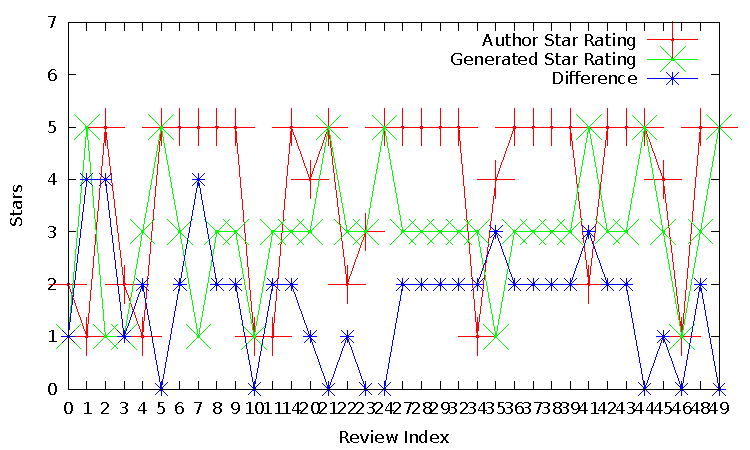
\includegraphics[width=0.8\textwidth]{data/pmi-free.pdf}
	\caption{PMI-IR with free applications}
	\label{fig:pmi-free}
	\end{figure}

The results of our first experiment in which we calculated the semantic orientations of phrases based on Google's search engine hit counts are shown above. As can be seen above, our ability at that point to reasonably match an application reviewer's star-rating was quite poor. The average absolute error was 2.04 stars. This meant that, if the reviewer had rated an application with a 3-star rating, we would, on average, generate a star-rating of 1-star or 5-stars. This is not good.

To make sure that the magnitude of the absolute error was not artificial, we went through all the reviews for which our generated star-rating was off by 2 or more star-ratings. The only way in which the absolute error could have been artificial is if there were a significant number of reviews in our small test set of 50 reviews whose star-ratings did not match the sentiment of the review. Unfortunately, this was not the case, Our implementation of the PMI-IR method of generating sentiment scores was simply not good enough.

\newpage

	\section{Results: PMI-Concordance}
	
	\begin{figure}[H]
	\centering
	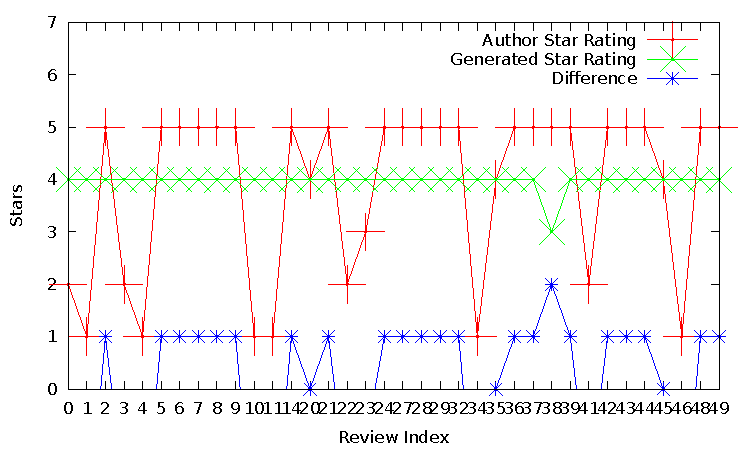
\includegraphics[width=0.8\textwidth]{data/pmi-cd-free.pdf}
	\caption{PMI-CD with free applications}
	\label{fig:pmi-cd-free}
	\end{figure}

	\begin{figure}[H]
	\centering
	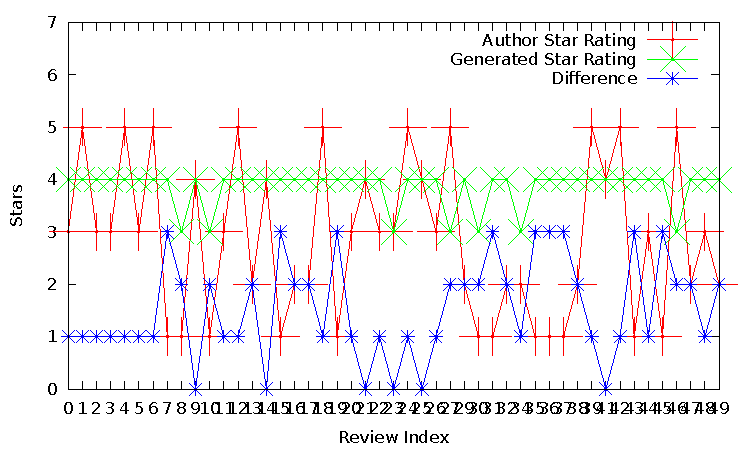
\includegraphics[width=0.8\textwidth]{data/pmi-cd-paid.pdf}
	\caption{PMI-CD with paid applications}
	\label{fig:pmi-cd-paid}
	\end{figure}

The results of our second experiment in which we calculated the semantic orientations of phrases based on the concordance of words in \textit{NLTK}'s \verb|movie_reviews| corpus are shown above. Unlike the PMI-IR experiment, we were able to obtain results for 50 full reviews from both the free application review corpus and the paid application review corpus. Thus, the results are a bit more meaningful.

Compared to our previous experiment, we were able to match the application reviewer's star-rating much better. It was still nowhere near as good as we would have liked, especially given that the expanded data set we worked with had no incongruities between star-ratings and reviews as before. The average absolute error when generating a star-rating over the subset of free reviews was 1.39 stars. The average absolute error when generating a star-rating over the subset of paid reviews was 1.39 stars.
	

\section{Results: Hierarchical Classification}

	\subsection{Characterisation of Corpora} 

	\begin{figure}[H]
	\centering
	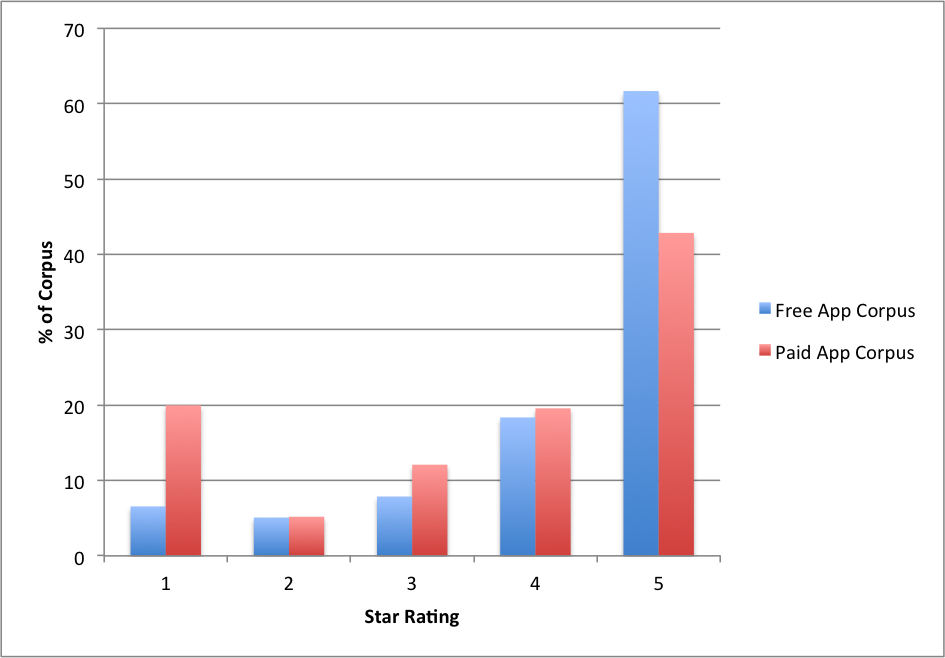
\includegraphics[width=0.8\textwidth]{data/dist_corpora.png}
	\caption{The distribution of star-ratings among reviews in each corpus}
	\label{fig:pmi-hc-corp-dist}
	\end{figure}

In our last set of experiments, we used the entirety of both review corpora to obtain our results. In the process of doing so we characterized the contents of the corpora for the sake of obtaining more accurate results. What follows is our characterization of the test set. As shown above, our test set has a tremendous number of positive reviews. If we were to guess a star-rating between 3 and 5, we would be correct most of the time. It is interesting to note that reviewers seemed more willing to assign 5-star-ratings to free applications and more willing to assign 1-star ratings for paid applications. This may be indicative of how forgiving people are of the quality of an application based on its cost. As the total number of reviews from both corpora numbers only 2,969, it is not really possible to make sweeping sociological remarks based on the figure shown above. 	


	\begin{figure}[H]
	\centering
	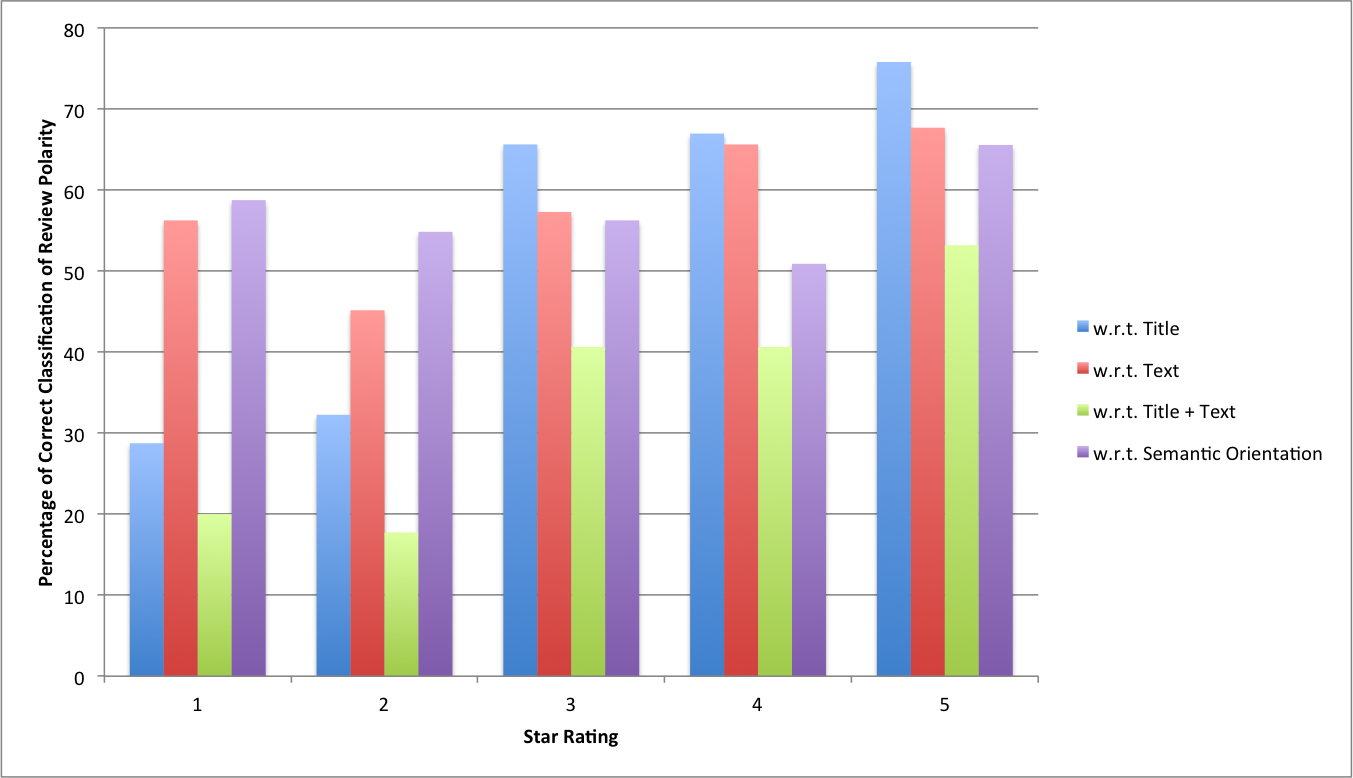
\includegraphics[width=0.8\textwidth]{data/pmi-cue-free-pol-acc.png}
	\caption{Accuracy with which different indicators produced correct review polarity from free app corpus.}
	\label{fig:pmi-cue-free-pol-acc}
	\end{figure}

	\begin{figure}[H]
	\centering
	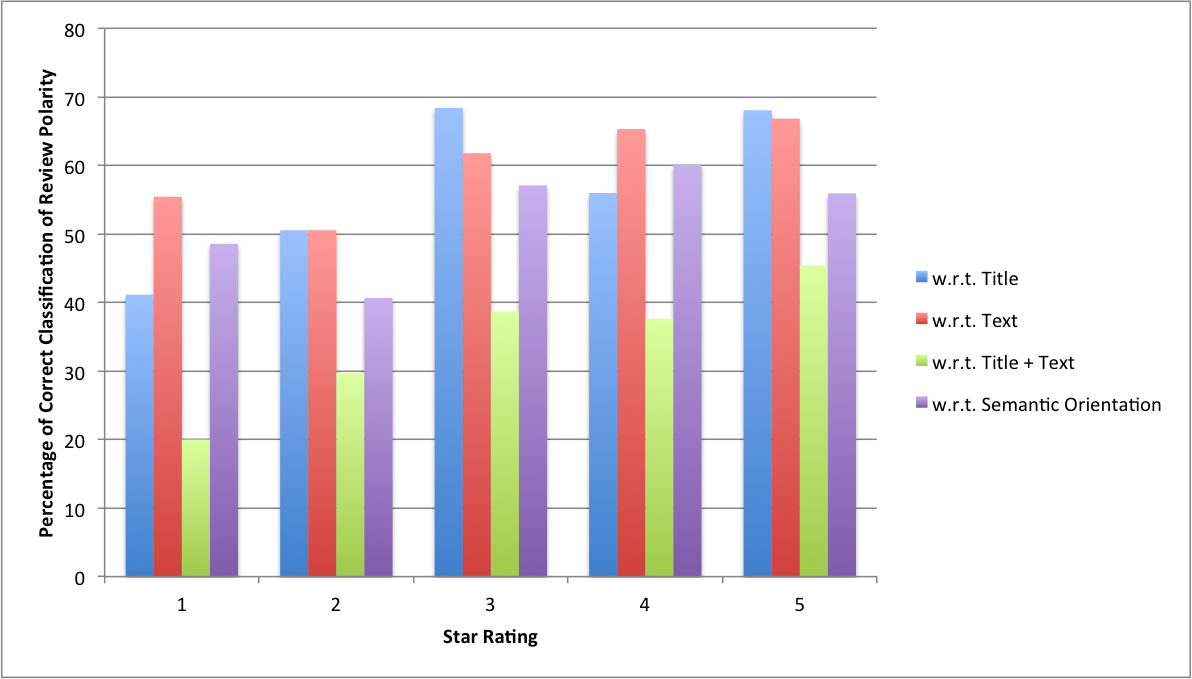
\includegraphics[width=0.8\textwidth]{data/pmi-cue-paid-pol-acc.png}
	\caption{Accuracy with which different indicators produced correct review polarity from paid app corpus.}
	\label{fig:pmi-cue-paid-pol-acc}
	\end{figure}

In order to accurately generate star-ratings for reviews, we had to be able to accurately determine the polarity of a review. To determine the best indicator of a review's polarity, we compared the star-rating assigned by the reviewer to four different indicators: the polarity of a review's title, the polarity of a review's text, the polarity of both the review's title and text if they were the same, and the calculated semantic orientation of the review's text. As shown above, the polarity of a review's text is the best indicator on average of a review's polarity. At first, we mistakenly believed that the title was a better indicator of the overall polarity of a review, but, after collecting and analyzing the data, we came to the correct conclusion. The result was a much better star-rating generator. 

Since our goal was not to model what star-ratings reviwers assign to mobile applications but to instead be able to generate star-ratings uniformly based on the sentiment of the text of a review, we decided to assess the accuracy of our star-rating generation a bit differently. To assess the accuracy of our hierarchical classifier, we first determined how well our generated star-ratings matched up to each review's original star-rating by star-rating. The accuracy for each star-rating was granted equal weight and averaged together to determine our overall accuracy. Then, we assessed the validity of this value by getting a sense of how well reviewers classified their own reviews into a star-rating.


\subsection{Classification with Empirically Defined SO-value Thresholds}
\label{subsection:empirically_defined_so}
\begin{figure}[H]
	\centering
	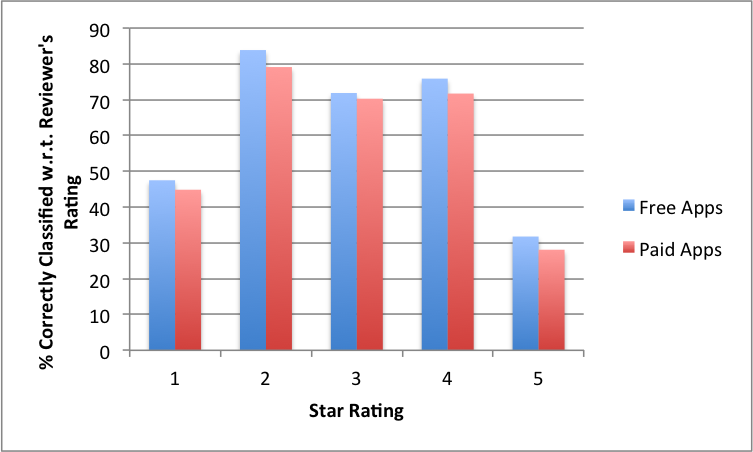
\includegraphics[width=0.8\textwidth]{data/pmi-cue-accuracy.png}
	\caption{Accuracy of generated star-ratings w.r.t star-ratings of original reviewers.}
	\label{fig:pmi-cue-acc}
	\end{figure}

The results shown above were obtained as described in Section 2.5.1. The polarity of each review was determined by the polarity of review's text and the threshold values for the star ratings were obtained via the same crude method used in previous experiments. The results above show a clear, vast improvement over our other attempts to generate star-ratings. Using these empirically defined thresholds, we achieved  an accuracy of 46.6\% for the free applications and 47.7\% for the paid applications.  

\newpage

		\subsection{Classification using Support Vector Machines}

%%% FREE APPS REVIEWS %%%
\begin{figure}[h!]
\centering
\subfigure[Results of Positive Reviews]{
	%%% FREE, POSITIVE %%%
    \begin{tabular*}{0.45\textwidth}{ l l  l  l }
 \hline
\multicolumn{4}{c}{Free Applications} \\ \hline \hline
\multicolumn{4}{c}{Positive Reviews (Rating: $\geq 3$)} \\
    \hline \hline
    	 Accuracy & Precision & Recall & F1-score \\ \hline
	0.70 & 0.49 & 0.70 & 0.58 \\ \hline
    \hline
    \end{tabular*}
	\label{fig:results_free_pos}
}
\subfigure[Results of Negative Reviews]{
	%%% FREE NEGATIVE %%%
    \begin{tabular*}{0.45\textwidth}{ l l  l  l }
 \hline
\multicolumn{4}{c}{Free Applications} \\ \hline \hline
\multicolumn{4}{c}{Negative Reviews (Rating: $\leq 3$)} \\
    \hline \hline
    	 Accuracy & Precision & Recall & F1-score \\ \hline
	0.58 & 0.57 & 0.96 & 0.72 \\ \hline
    \hline
    \end{tabular*}
	\label{fig:results_free_neg}
}
%\caption[Optional caption for list of figures]{10-fold Cross Validation Results for Positive \subref{fig:subfig1} and Negative \subref{fig:subfig2} Reviews}
\caption[Optional caption for list of figures]{10-fold Cross Validation Scores and Accuracy Measures for Free Applications }
\label{fig:analysis_free}
\end{figure}
%%% END FREE APPS REVIEWS %%%

\paragraph{Free Applications} For the dataset containing the free applications, we observe that the accuracy for is higher for the \textit{positive} reviews compared to the \textit{negative} reviews. The precision scores for both \textit{positive} and \textit{negative} reviews are comparable at around 50\%, but the largest difference affecting the F1-score is the recall score, which is much higher for \textit{negative} reviews.

%%% PAID APPS REVIEWS %%%
\begin{figure}[h!]
\centering
\subfigure[Results of Positive Reviews]{
	%%% FREE, POSITIVE %%%
    \begin{tabular*}{0.45\textwidth}{ l l  l  l }
 \hline
\multicolumn{4}{c}{Paid Applications} \\ \hline \hline
\multicolumn{4}{c}{Positive Reviews (Rating: $\geq 3$)} \\
    \hline \hline
    	 Accuracy & Precision & Recall & F1-score \\ \hline
	0.57 & 0.33 & 0.57 & 0.42 \\ \hline
    \hline
    \end{tabular*}
	\label{fig:analysis_paid_pos}
}
\subfigure[Results of Negative Reviews]{
	%%% FREE NEGATIVE %%%
    \begin{tabular*}{0.45\textwidth}{ l l  l  l }
 \hline
\multicolumn{4}{c}{Paid Applications} \\ \hline \hline
\multicolumn{4}{c}{Neg Reviews (Rating: $\leq 3$)} \\
    \hline \hline
    	 Accuracy & Precision & Recall & F1-score \\ \hline
	0.79 & 0.79 & 1.00 & 0.88 \\ \hline
    \hline
    \end{tabular*}
	\label{fig:analysis_paid_neg}
}
\caption[Optional caption for list of figures]{10-fold Cross Validation Scores and Accuracy Measures for Paid Applications }
\label{fig:subfigureExample}
\end{figure}
%%% END PAID APPS REVIEWS %%%

\paragraph{Paid Applications} For the dataset containing the paid applications, we observe that the accuracy for is higher for the \textit{negative} review compared to the \textit{positive} reviews. The scores and accuracy measures for the \textit{negative} reviews indicate the classifier performs much better overall with negative reviews.

%%% COMBINED APPS REVIEWS %%%
\begin{figure}[h!]
\centering
\subfigure[Results of Positive Reviews]{
	%%% FREE, POSITIVE %%%
    \begin{tabular*}{0.45\textwidth}{ l l  l  l }
 \hline
\multicolumn{4}{c}{Combined Free \& Paid Applications} \\ \hline \hline
\multicolumn{4}{c}{Positive Reviews (Rating: $\geq 3$)} \\
    \hline \hline
    	 Accuracy & Precision & Recall & F1-score \\ \hline
	0.63 &0.40 &0.63 & 0.49 \\ \hline
    \hline
    \end{tabular*}
	\label{fig:subfig1}
}
\subfigure[Results of Negative Reviews]{
	%%% FREE NEGATIVE %%%
    \begin{tabular*}{0.45\textwidth}{ l l  l  l }
 \hline
\multicolumn{4}{c}{Combined Free \& Paid Applications} \\ \hline \hline
\multicolumn{4}{c}{Neg Reviews (Rating: $\leq 3$)} \\
    \hline \hline
    	 Accuracy & Precision & Recall & F1-score \\ \hline
	0.74 & 0.74 & 1.00 & 0.85 \\ \hline
    \hline
    \end{tabular*}
	\label{fig:subfig2}
}
\caption[Optional caption for list of figures]{10-fold Cross Validation Scores and Accuracy Measures for Both Applications}
\label{fig:subfigureExample}
\end{figure}
%%% END COMBINED APPS REVIEWS %%%

\paragraph{Mixed Dataset} When trained on a combined dataset containing a mixture of free and paid application user reviews, the classifier appears to perform better on classifying \textit{negative} reviews than \textit{positive} reviews. The accuracy, precision, recall and F1-scores for the classifier on \textit{negative} reviews all outperform that of the classifier on \textit{positive} reviews. The precision score for \textit{positive} reviews are particularly low.

\begin{figure}[H]
	\centering
	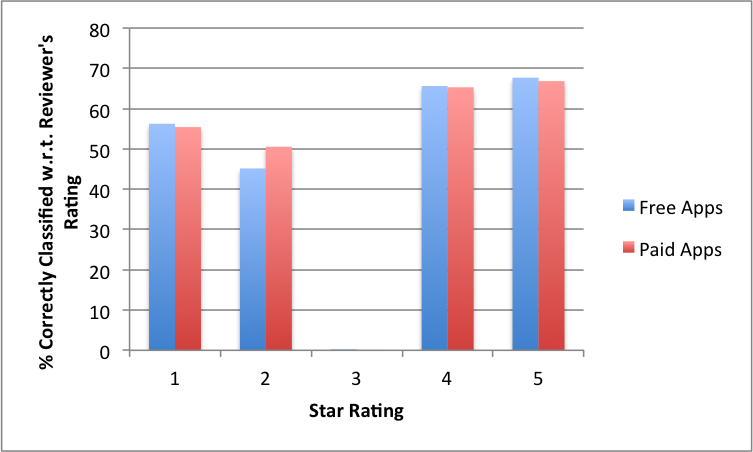
\includegraphics[width=0.7\textwidth]{data/pmi-cue-acc-wsvm.png}
	\caption{Accuracy of generated star-ratings w.r.t star-ratings of original reviewers.}
	\label{fig:pmi-cue-wsvm-acc}
	\end{figure}

\paragraph{Overall Performance}
We obtained 4 different classifiers by using the trained SVMs, resulting in two hierarchical classifiers per application group (free/paid). We then ran similar benchmarks to those performed on the empirically defined SO-threshold hierarchical classifier from Section~\ref{subsection:empirically_defined_so}. We achieved improved accuracy rates of 60.1\% for free applications and 55.1\% for paid applications. It is noted that our classifier performs best near the extremities of the star-rating scale, with few 3-star rating reviews correctly identified.

\section{Selected Examples}
\subsection{Star-rating Prediction on Filtered Dataset}
TODO: Filtered dataset refer to \verb|datasets/datadataset_accurate_free.dat| and \verb|data/dataset_accurate_paid.dat|, and mean that they have consistent and logical review-text to star-ratings. We need to show case a 1-star review and 5-star review and how the polarity and so and classification accurately predicts the star rating.

\chapter{Analysis}
	\section{PMI-IR}

As far as we know, the PMI-IR method is a perfectly reasonable method for generating star-ratings. Unfortunately, the tiny amount of data we were able to obtain did not provide us with enough data to make a good model for generating star-ratings accurately. Previous work has shown that this method produces promising results \cite{Turney2001}. This work was performed almost a decade ago, however, and search engines have become far more sensitive to automatic queries. To collect enough data to accurately assess and use the PMI-IR method would require either intimate access to a search engine's inner workings or enough time to manually obtain all the hit counts required from the browser interface to a search engine. Either way, this method was not a good fit for our project and it was good that we discovered this early.

	\section{PMI-Concordance}

As far as we know, the PMI-Concordance method is also a perfectly reasonable method for generating star-ratings. When the PMI-IR method did not pan out, we decided to try to replace hit counts for concordance values. To keep the amount of time it took to calculate the semantic orientation for a single word based on concordance low, we only considered the first 20 or so occurences of a word whose semantic orientation we were calculating in \textit{NLTK} 's \verb|movie_review| database. The window of words we used around the word whose semantic orientation we were calculating was only about 20 words in either direction. Perhaps if we had used all occurences of a word in the movie reviews and a window of words that spanned the whole corpus, we would have been able to produce better results. Such an approach would have been prohibitively time-consuming, however. As we did not obtain good results by using this method to generate star-ratings, we discarded it in favor of another. 


	\section{Hierarchical Classification}
	\subsection{Using Empirically Defined SO-Value Thresholds}
The empirically defined thresholds performs well on star-rating estimations away from the extremities. As such, it was more accurate in predicting ratings of 2, 3 and 4, achieving accuracy results of well over 70\% for them. For predicting extreme star-ratings, such as 1 and 5, it fairs poorly, with values consistently less than 50\%.

	\subsection{Using SVM as Classifiers} 
\subsubsection{SVM Classification Performance}
When the polarity of a review is accurately classified, using SVMs to classify the SO-values showed promise. Accuracy was consistently above 50\% across free and paid applications for both positive and negative reviews. It is also worthy to note that for free applications, classifying positive reviews does better than negative reviews but the opposite is true for paid applications. This might indicate some intrinsic properties in terms of the type of reviews that people leave which differ across free and paid applications. The F1-scores for negative reviews were consistently higher than positive reviews across free and paid applications, which might also indicate some bias of negative reviewers being more objective in assigning star-ratings.
\subsubsection{Overall Performance}
It would appear that the SO-values are good in helping to steer accuracy of ratings towards the extremities, but do not have enough significance in classifying data towards a more neutral star-rating. This might indicate a need for a richer feature set in order to accurately discern small differences in star-ratings. 

	\section{Noisy Training and Test Data}
\subsection{Inconsistent Reviews and Ratings from Users}

One difficulty in learning from training examples, and one of the motivations of this work is that the users often give star ratings that do not match their text review. This adds noise to the training set, making accurate prediction very difficult. The only sure way around this is to carefully hand-tag the reliable reviews in the training set. Features such as \'Was this review helpful?\' implemented in Amazon and few other review sites might help in determining the stable training sets, as this feature will allow the system to recognize reviews with less noise. But there was no such feature in the Google app store.

The following are some examples of cases where user ratings do not match the contents.

\begin{table}[h]
	\centering
    \begin{tabularx}{\textwidth}{ l | l | l |  l | X}
    \hline\hline
		Price  & Index & User Rating & Title & Text Review\\ 
    \hline
		Paid & 1678 & 5.0 & It won't work & I can click on app but it.just flashes the screen then nothing doesn't go into app...maybe my phone but idk... but whatev i got.it for .99 pennies ...save.for when i get tablet... skeet skeet skeet \\
		Paid & 1143 & 2.0 & One of the best & Entertaining and fun I always play it. Its worth the money \\
		Free & 1189 & 5.0 & Gets boring & To easy to make money I literally have 3 million dollars that I can't use. \\
		Free & 666 & 1.0 & Awesome.... & But I hve some probs....it slows down always...plzz fix it for htc one v \\
    \hline
    \end{tabularx}
\caption{Examples of user rating/content mismatch}
\label{fig:postags}
\end{table}

\chapter{Conclusion}

\section{Conclusion}
There is an often unaddressed need to make sure that customers classify their reviews correctly. There are reviewers out there who, for whatever reason, incorrectly assign their reviews for a product or service a much higher or lower rating than the meat of their review would have you believe is deserved. There is a sizable body of published work out there that describe projects with the aim of determining whether or not a review is positive or negative based on the underlying sentiment of text. In that body of literature, there are very few endeavors that seek to classify a passage of text as positive, negative or neutral. We sought to do much more than that. We sought to classify reviews along the 5-star spectrum. Not only that, but we strove to make the star-ratings we generated classify the reviews better than star-ratings that reviewers themselves assigned. This was a large undertaking and, given the constraints on this work, we obtianed reasonable results. We tried many methods of generating star-ratings and stumbled upon one that works quite well. Our moderate success shows that this direction holds promise, and our pitfalls showed that there is much more work to be done and avenues to be explored. 

\section{Limitations \& Future Work}
In this section, we outline aspects of the project that could be extended upon and how we hypothesize they would improve results. 
\subsection{Improving Polarity Detection}
The first step in the hierarchical classification is to detect the polarity of the review text in question into \textit{positive} or \textit{negative}. As we showcased, this step is important as it also determines the subsequent SVM model used to classify the review into exact star-ratings.
\subsubsection{More Features for Naive Bayes Polarity Classifier}
 In our implementation, we made use of a Bag-of-Words (BOW) model over feature sets created from the \textit{NLTK} \verb|movie_reviews| corpus. However, we suspect that using other features to classify the polarity of the text might work better, such as using the length of the text, number of fully-capitalized words and number of exclamation marks used. We could create feature vectors of each of these individual features and train them on the corpus. This would likely improve polarity detection.
\subsection{Improving Semantic-Orientation Estimation}
Semantic-orientation (SO) is based on the Pointwise Mutual Information (PMI) values, which have been shown to be difficult to calculate and require estimators. We implemented and show-cased online methods (PMI-IR), and offline methods (PMI-Concordance, PMI-CUE). The PMI-IR method outlined has had positive results, but is limited due to restrictions placed by search engine providers and also by the lack of transparency required to verify the accuracy of the results. The PMI-Concordance method showed positive results,  but runs slowly. The PMI-CUE method showed the most promise in terms of accuracy and speed.
\subsubsection{Using n-gram Models}
The PMI-CUE method of estimating the SO-values lies on creating probability distributions on words. However, it does not take into account the order of the words, so \verb|SO("very", "annoying")| and \verb|SO("annoying", "very")| will return the same results. It also assumes independence of the words appearing together. By using a bigram or trigram model, we would be able to take word order into account, and also have a better approximation of the co-occurrences of each phrase consisting of 2 words.

\subsection{Improving SVM classification}
The Support Vector Machines (SVM) were used to identify the exact star-ratings based on the SO-values of a given text. However, we noted that the SO-values did not have a distinct enough variation in order to accurately distinguish between some of the star-ratings.

\subsubsection{Richer Features}
Instead of just using the SO-value of the text as the only feature set, we could also take into account the SO-value of the title, and other aspects of a review into having a richer feature set. We suspect that this would enable the classifiers to distinguish between two star-ratings on the same side of polarity with much greater accuracy.

\subsection{Better Datasets}
The system structure relies heavily on the availability of datasets in order to work well. We outline some aspects of data collection which would likely improve ease and accuracy of the results.

\subsubsection{Easier Collection Methods}
It would be ideal if the Google Play Store provided official APIs to enable us to query and extract information from their store. Manual collection is slow, and results in a much smaller set of data due to time and logistical constraints. 

\subsubsection{Less Noise}
As outlined, some of the reviews by users have huge discrepancies in their assigned star-ratings and the contents and sentiments of their reviews. This makes testing and validation difficult under time and logistical constraints. 

\section{Closing Remarks}
Sentiment analysis of text is a difficult task, more so in the context of user reviews. The language used by reviewers varies greatly across domains, making it difficult to have a single system or method of analyzing sentiments. However, we have showcased a framework which has positive results, which can also be naturally extended to fit reviews across different domains. We achieved excellent progress in determining sentiment and polarity, both using supervized and unsupervized methods. We expect that the system and results shown will aid in improving the fields of sentiment analysis for the future.

%\bibliographystyle{plain}
\bibliographystyle{ieeetr}
\bibliography{references}

\end{document}
